%=============================================================================
\subsection{Principaux choix de réalisation}
%=============================================================================

Ce rapport présente les choix techniques et les détails d'implémentation du compilateur et interpréteur MiniJaja développé dans le cadre du projet de Génie Logiciel. Le document couvre l'ensemble du pipeline de traitement, depuis l'analyse lexicale et syntaxique via ANTLR jusqu'à l'interprétation de l'arbre syntaxique abstrait (AST).

\subsubsection{Architecture Générale}

L'architecture du projet suit un modèle en pipeline composé de quatre phases principales :

\begin{enumerate}
    \item \textbf{Analyse Lexicale/Syntaxique} : Génération du CST via ANTLR4
    \item \textbf{Construction de l'AST} : Transformation du CST en AST via le pattern Visitor
    \item \textbf{Analyse Sémantique} : Vérification des types et des déclarations
    \item \textbf{Interprétation} : Exécution de l'AST via un Walker en parcours préfixe
\end{enumerate}

\begin{figure}[h]
\centering
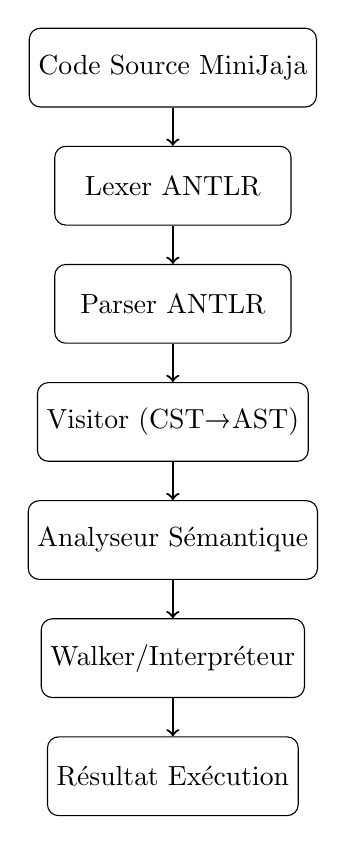
\begin{tikzpicture}[
    node distance=1.5cm,
    box/.style={rectangle, draw, rounded corners, minimum width=3cm, minimum height=1cm, text centered},
    arrow/.style={->, thick}
]
    \node[box] (source) {Code Source MiniJaja};
    \node[box, below of=source] (lexer) {Lexer ANTLR};
    \node[box, below of=lexer] (parser) {Parser ANTLR};
    \node[box, below of=parser] (visitor) {Visitor (CST→AST)};
    \node[box, below of=visitor] (semantic) {Analyseur Sémantique};
    \node[box, below of=semantic] (walker) {Walker/Interpréteur};
    \node[box, below of=walker] (result) {Résultat Exécution};
    
    \draw[arrow] (source) -- (lexer);
    \draw[arrow] (lexer) -- (parser);
    \draw[arrow] (parser) -- (visitor);
    \draw[arrow] (visitor) -- (semantic);
    \draw[arrow] (semantic) -- (walker);
    \draw[arrow] (walker) -- (result);
\end{tikzpicture}
\caption{Pipeline de compilation/interprétation MiniJaja}
\end{figure}

%=============================================================================
\subsection{Du code source au CST (contexte)}
%=============================================================================

Le pipeline s'appuie sur ANTLR4 pour produire un CST (Concrete Syntax Tree) à partir du code source, puis un Visitor transforme ce CST en AST (Abstract Syntax Tree) propre au projet.

\subsubsection{Rôle d'ANTLR côté analyse lexicale (Lexer)}

ANTLR découpe d'abord le \textbf{flux de caractères} en \textbf{lexèmes} et les transforme en \textbf{tokens} typés (ex : mot-clé, identifiant, entier, opérateur, séparateur). Chaque token transporte des \textbf{métadonnées de localisation} (ligne/colonne) utilisées ensuite pour attacher une position source aux nœuds de l'AST.

\medskip
\noindent\textbf{En pratique :}
\begin{itemize}
    \item le \emph{lexer} applique des règles lexicales (expressions régulières) pour reconnaître les unités du langage ;
    \item les espaces et commentaires sont ignorés ou envoyés sur un canal caché ;
    \item le \emph{parser} consomme la suite de tokens pour produire un CST (arbre de règles) cohérent avec la grammaire.
\end{itemize}

\medskip
\noindent\textbf{Périmètre de ce rapport.} Les détails de la grammaire ANTLR et du diagnostic complet des erreurs syntaxiques ne sont pas le cœur du document : on se concentre ensuite sur \textbf{(1) la construction de l'AST} et \textbf{(2) l'interprétation de l'AST} (Walker + mode debug), ainsi que sur les erreurs/exceptions associées à ces deux phases.

%=============================================================================
\subsection{Construction de l'Arbre Syntaxique Abstrait (AST)}
%=============================================================================

\subsubsection{Le Pattern Visitor pour la transformation CST→AST}

La transformation du CST (Concrete Syntax Tree) généré par ANTLR vers notre AST personnalisé est réalisée via le pattern Visitor implémenté dans \texttt{MiniJajaInterpreterVisitor}.

Le Visitor applique une correspondance \emph{règle de grammaire} $\rightarrow$ \emph{nœud métier}. Chaque nœud créé peut recevoir une \texttt{SourcePosition} (fichier/ligne/colonne) extraite du token de début de la règle ANTLR, ce qui rend les erreurs ultérieures (construction/interprétation) \textbf{localisables}.

\subsubsection{Stratégie de construction : règles → noeuds et listes chaînées}

La grammaire ANTLR produit un arbre de règles. Le Visitor opère une \textbf{projection} : chaque règle pertinente retourne un \texttt{AstNode} métier.

\begin{itemize}
    \item \textbf{Noeuds structurels} : \texttt{ClasseNode} (racine), \texttt{MainNode}, \texttt{MethodeNode}.
    \item \textbf{Listes récursives} : plusieurs listes sont représentées sous forme de \emph{chaînes} (liste + reste). C'est visible pour :
    \begin{itemize}
        \item \texttt{DeclsNode} (déclarations globales : variables, constantes, tableaux, méthodes),
        \item \texttt{VarsNode} (variables locales),
        \item \texttt{EntetesNode} (paramètres),
        \item \texttt{InstructionsNode} (suite d'instructions),
        \item \texttt{ListExpNode} (arguments d'appel).
    \end{itemize}
\end{itemize}

Ce choix simplifie le Visitor : on construit la tête, puis on enchaîne le reste (ou \texttt{null}/noeud vide) et l'interpréteur peut traiter récursivement la structure.


\subsubsection{Erreurs de construction d'AST (Visitor)}

Le Visitor est volontairement strict : si un cas de grammaire n'est pas géré, l'exécution doit échouer tôt.

\noindent\textbf{Exemples typiques d'échec (sans extrait de code) :}
\begin{itemize}
    \item une règle d'instruction non prise en charge entraîne une \texttt{IllegalStateException} ;
    \item un nœud ANTLR inattendu dans le parcours déclenche une \texttt{UnsupportedOperationException} ;
    \item des garde-fous de cohérence CST peuvent lever une \texttt{RuntimeException} (ex : instruction \texttt{ecrire} sans opérande reconnu).
\end{itemize}

\noindent\textbf{Exceptions de construction AST :}
\begin{itemize}
    \item \texttt{IllegalStateException} : règle d'instruction non prise en charge (visitor incomplet).
    \item \texttt{UnsupportedOperationException} : nœud ANTLR inattendu dans le parcours (signal d'écart grammaire/visitor).
    \item \texttt{RuntimeException} : états impossibles (ex: \texttt{WRITE} sans identifiant ni chaîne) — garde-fous de cohérence CST.
\end{itemize}

\subsubsection{Hiérarchie des Noeuds AST}

Tous les noeuds de l'AST héritent de la classe abstraite \texttt{AstNode} qui définit l'interface commune :

\noindent\textbf{Contrat minimal :}
\begin{itemize}
    \item une représentation \texttt{toStringTree()} ;
    \item un accès aux enfants via \texttt{getChildren()} (utile au Walker) ;
    \item une exécution via \texttt{interpret(Stacks)} (souvent vide par défaut) ;
    \item pour les expressions, une évaluation via \texttt{evaluate(Stacks)}.
\end{itemize}

\subsubsection{Classification des nœuds AST (tableau récapitulatif)}

Le tableau suivant regroupe les nœuds par \textbf{familles comportementales} et explicite, pour chaque famille, les \textbf{attributs structurants} (références vers sous-nœuds, identifiants, types) ainsi que les \textbf{méthodes clés} utilisées à l'exécution.

\begin{longtable}{|p{2.8cm}|p{3.4cm}|p{6.4cm}|p{3.0cm}|}
\caption{Groupes de nœuds AST : rôle, attributs et méthodes}\label{tab:groupes-nodes}\\
\hline
    \textbf{Groupe} & \textbf{Exemples} & \textbf{Attributs principaux (idée)} & \textbf{Méthodes clés} \\
\hline
\endfirsthead
\hline
    \textbf{Groupe} & \textbf{Exemples} & \textbf{Attributs principaux (idée)} & \textbf{Méthodes clés} \\
\hline
\endhead
Structurels & \texttt{ClasseNode}, \texttt{MainNode}, \texttt{MethodeNode}, \texttt{DeclsNode}, \texttt{VarsNode}, \texttt{EntetesNode}, \texttt{InstructionsNode} &
Références vers listes chaînées (tête + reste), identifiants de méthodes, variables de classe, sous-arbres \emph{vars/instrs/decls/entêtes}. &
    \texttt{interpret}, \texttt{getChildren}, \texttt{toStringTree} \\
\hline
Déclarations & \texttt{VarNode}, \texttt{CstNode}, \texttt{TableauNode}, \texttt{EnteteNode} &
    \textbf{Type} déclaré, \textbf{identifiant}, éventuelle \textbf{expression d'initialisation} (ou taille pour tableau). &
    \texttt{interpret} (déclare dans \texttt{Stacks}), \texttt{getChildren} \\
\hline
Instructions & \texttt{AffectationNode}, \texttt{SiNode}, \texttt{TantqueNode}, \texttt{AppelINode}, \texttt{RetourNode}, \texttt{EcrireNode}, \texttt{IncrementNode}, \texttt{SommeNode} &
Cibles (identifiant / accès tableau), expressions, sous-listes d'instructions (then/else, corps de boucle), informations d'appel (ident + arguments). &
    \texttt{interpret} (effets), parfois réécriture via \texttt{setChildren} / remise à zéro des enfants \\
\hline
Expressions & \texttt{IdentNode}, \texttt{TabNode}, \texttt{NbreNode}, \texttt{BoolValueNode}, \texttt{PlusNode}, \texttt{MinusNode}, \texttt{AndNode}, \texttt{NotNode}, \texttt{AppelENode} &
Opérandes gauche/droite, identifiants, index, littéraux, arguments d'appel. Les types sont \emph{dynamiques} à l'exécution. &
    \texttt{evaluate} (renvoie une valeur), \texttt{getChildren} \\
\hline
Retrait (cleanup) & \texttt{rVar}, \texttt{rVars}, \texttt{rDeclrs}, \texttt{rEntetes}, \texttt{RestoreContextNode} &
Référence vers le nœud ou la liste à nettoyer ; pour \texttt{RestoreContextNode}, le nom de la méthode/contexte. &
    \texttt{interpret} (retire dans \texttt{Stacks}, et/ou \texttt{popContext}) \\
\hline
\end{longtable}

%=============================================================================
\subsection{Note sur l'analyse sémantique (hors focus)}
%=============================================================================

Le projet contient une analyse sémantique (déclarations, compatibilités de types, validation d'appels de méthodes). Elle est essentielle au pipeline global, mais le présent rapport reste centré sur :
\begin{enumerate}
    \item la construction de l'AST (Visitor),
    \item l'interprétation (Walker + exécution des nœuds),
    \item les erreurs/exceptions associées à ces deux étapes.
\end{enumerate}

\noindent Les erreurs sémantiques (doublons, portées, types statiques) sont donc volontairement peu détaillées ici.

%=============================================================================
\subsection{Interprétation}
%=============================================================================

\subsubsection{Le Walker : Parcours de l'AST}

L'interprétation est réalisée par un parcours préfixe (preorder) de l'AST via la classe \texttt{Walker} :

\noindent\textbf{Principe d'exécution :}
\begin{itemize}
    \item le Walker visite le nœud courant (compteur interne incrémenté) ;
    \item si le debug est actif, il peut \textbf{interrompre} l'exécution \emph{avant} l'interprétation du nœud ;
    \item le Walker exécute \texttt{interpret(stacks)} ;
    \item puis visite les enfants fournis par \texttt{getChildren()}.
\end{itemize}

\subsubsection{Mode Debug : pas à pas et points d'arrêt}

Le Walker délègue le \emph{contrôle d'exécution} à une instance \texttt{Debug}. Le principe est le suivant : \textbf{avant} d'exécuter un nœud (donc avant \texttt{node.interpret(stacks)}), le Walker appelle \texttt{debug.beforeNode(...)}.

\begin{itemize}
    \item En mode \textbf{DISABLED}, aucune pause n'est possible.
    \item En mode \textbf{STEP\_BY\_STEP}, une pause est déclenchée à chaque nœud.
    \item En mode \textbf{BREAKPOINTS}, une pause n'est déclenchée que si le compteur interne (\texttt{lineCounter}) correspond à un breakpoint.
\end{itemize}

\noindent\textbf{Décision de pause (sans extrait de code) :}
\begin{itemize}
    \item si le mode est \textbf{DISABLED}, l'exécution continue ;
    \item si le mode est \textbf{STEP\_BY\_STEP}, on pause à chaque nœud ;
    \item si le mode est \textbf{BREAKPOINTS}, on pause uniquement quand le compteur correspond à un point d'arrêt ;
    \item pendant la pause, une boucle interactive lit une commande utilisateur (continuer, step, dump mémoire, etc.).
\end{itemize}

La pause est interactive (lecture sur l'entrée standard) et permet d'inspecter la mémoire. Dans notre cas, cette fonctionnalité est pensée comme une \textbf{aide au débogage de l'interprétation} : le programme s'arrête avant un nœud, on observe l'état de la pile, puis on reprend.

\noindent\textbf{Fonctions debug disponibles :}
\begin{itemize}
    \item \textbf{Avancer} (step) : exécuter le prochain nœud puis repasser en pause.
    \item \textbf{Continuer} (continue) : exécuter sans pauses jusqu'à la fin.
    \item \textbf{Afficher la table des symboles} : état des identifiants connus.
    \item \textbf{Gérer les breakpoints} : ajouter/supprimer une étape.
\end{itemize}

\subsubsection{Memoir et Interpretation:}

La classe \texttt{Stacks} implémente la mémoire d'exécution avec une structure de pile classique :

Chaque entrée mémoire peut être vue comme un quadruplet \emph{(identifiant, valeur, catégorie d'objet, type)} :
\begin{itemize}
    \item \textbf{identifiant} : nom logique (éventuellement scopé) ;
    \item \textbf{valeur} : valeur courante (entier, booléen, structure tableau, etc.) ;
    \item \textbf{catégorie} : \texttt{var}/\texttt{cst}/\texttt{tab}/\texttt{meth} ;
    \item \textbf{type} : type MiniJaja associé.
\end{itemize}

\subsubsection{Gestion des Contextes pour la Récursivité}

La pile supporte les appels récursifs grâce à un système de contextes :

Lors d'un appel, on empile un \textbf{suffixe de contexte} (nom de méthode + indice de récursivité si besoin). Les variables/paramètres peuvent alors être distingués par un nom de la forme \texttt{nom@contexte}.

\medskip
\noindent\textbf{Exemple d'effet :} si \texttt{f} s'appelle récursivement, on peut obtenir \texttt{x@f}, puis \texttt{x@f1}, \texttt{x@f2}, etc. Cela permet au retrait (nettoyage) et aux accès variables de viser la bonne instance.

\subsubsection{Interprétation des Noeuds Principaux}

\subsubsection{ClasseNode}

Le noeud racine déclare la variable de classe utilisée pour le retour de fonctions :

\noindent\textbf{Rôle :} initialiser une ``variable de classe'' dédiée au mécanisme de retour (valeur de \texttt{return} récupérée lors d'un appel de fonction).

\subsubsection{VarNode - Déclaration de Variable}

\noindent\textbf{Rôle :} déclarer une variable dans \texttt{Stacks} (nom possiblement scopé en contexte de méthode), avec une valeur initiale si une expression est fournie, sinon une valeur par défaut.

\subsubsection{AffectationNode - Affectation}

\noindent\textbf{Rôle :} affecter une valeur évaluée à une cible (variable ou tableau). Le nœud effectue une \textbf{vérification dynamique de type} et peut lever une exception si la valeur n'est pas compatible.

\noindent\textbf{Erreur Runtime - Affectation :} \texttt{RuntimeException}: "Type error: cannot assign value of type \{valueType\} to variable \{varName\} of type \{varType\}"

\subsubsection{SiNode - Structure Conditionnelle}

Le \texttt{SiNode} modifie dynamiquement ses enfants selon l'évaluation de la condition :

\noindent\textbf{Rôle :} évaluer la condition (doit être booléenne) et sélectionner la branche à exécuter en \textbf{réécrivant la liste des enfants} visités ensuite par le Walker.

\noindent\textbf{Erreur Runtime - Condition :} \texttt{ClassCastException}: "If condition must evaluate to Boolean, got: \{type\}"

\subsubsection{TantqueNode - Boucle While}

Implémentation de la boucle par réécriture dynamique de l'arbre :

\noindent\textbf{Rôle :} si la condition est vraie, exécuter le corps puis \textbf{replanifier une itération} en injectant une nouvelle occurrence du nœud de boucle comme enfant ; sinon, arrêter la boucle (aucun enfant).

\subsubsection{AppelINode - Appel de Méthode}

L'appel de méthode gère la création du contexte et le passage de paramètres :

\noindent\textbf{Rôle :} préparer un appel (résolution de la méthode, évaluation des arguments, vérification arité), puis créer un \textbf{contexte} dans \texttt{Stacks} et injecter des nœuds enfants dans l'ordre : déclarations locales, instructions, retrait des variables, retrait des paramètres, restauration du contexte.

\noindent\textbf{Erreur Runtime - Appel de Méthode :} \texttt{RuntimeException}: "Appel de la méthode '\{methodName\}' : attendu \{expected\} argument(s), reçu \{received\}."

\subsubsection{RetourNode - Instruction Return}

\noindent\textbf{Rôle :} évaluer l'expression retournée et la stocker dans la variable de classe utilisée comme ``registre de retour''.

\noindent\textbf{Erreur Runtime - Return :} \texttt{RuntimeException}: "Erreur: Variable de classe non définie dans la pile"

\subsubsection{EcrireNode - Instruction d'Affichage}

\noindent\textbf{Rôle :} afficher une valeur (identifiant, expression ou accès tableau). Le nœud refuse l'affichage direct d'un tableau entier ou d'une référence de méthode.

\noindent\textbf{Erreur Runtime - Ecrire :} \texttt{RuntimeException}: "Type error: cannot print array directly or method reference"

\subsubsection{Évaluation des Expressions}

\subsubsection{Classe Expression}

Toutes les expressions implémentent la méthode \texttt{evaluate()} :

\noindent\textbf{Principe :} une expression renvoie une valeur (entier, booléen, etc.) et peut lever une exception en cas d'incompatibilité de types ou d'accès mémoire invalide.

\subsubsection{IdentNode - Référence de Variable}

\noindent\textbf{Rôle :} accéder à la valeur d'une variable. En contexte de méthode, l'accès privilégie un nom scopé \texttt{nom@contexte} si présent.

\subsubsection{Opérations Arithmétiques}

\noindent\textbf{Rôle :} évaluer les opérandes, vérifier qu'ils sont entiers, puis produire un entier.

\noindent\textbf{Erreurs Runtime - Opérations Arithmétiques :} \texttt{RuntimeException}: "Type error: both expressions must evaluate to Integer exp: \{left\} terme: \{right\}"

\subsubsection{Opérations Logiques}

\noindent\textbf{Rôle :} évaluer des booléens et produire un booléen (avec erreur si les opérandes ne sont pas booléens).

\noindent\textbf{Erreurs Runtime - Opérations Logiques :} \texttt{RuntimeException}: "Type error: both expressions must evaluate to Boolean"

\subsubsection{AppelENode - Appel de Fonction comme Expression}

\noindent\textbf{Rôle :} exécuter un appel de fonction et récupérer la valeur de retour depuis la variable de classe.

\noindent\textbf{Erreur Runtime - AppelE :} \texttt{RuntimeException}: "Erreur: appelE hors d'une classe"

\subsubsection{Noeuds de Retrait (Cleanup)}

Les noeuds \texttt{rXxx} gèrent le nettoyage de la pile après l'exécution :

\noindent\textbf{Principe :}
\begin{itemize}
    \item les listes (\texttt{VarsNode}, \texttt{DeclsNode}, \texttt{EntetesNode}) sont parcourues récursivement ;
    \item chaque déclaration est retirée de \texttt{Stacks} (en tenant compte du nom scopé en contexte de méthode) ;
    \item en fin d'appel de méthode, \texttt{RestoreContextNode} restaure le contexte (pop) pour revenir à l'appelant.
\end{itemize}
\newpage
%=============================================================================
\subsection{Synthèse des Erreurs et Exceptions (construction AST \& interprétation)}
%=============================================================================

\subsubsection{Deux familles d'échecs}

\begin{table}[h]
\centering
\begin{tabular}{|l|p{9.5cm}|}
\hline
    \textbf{Famille} & \textbf{Intention} \\
\hline
Construction AST (Visitor) & Détecter un décalage grammaire/visitor (cas non géré) ou un état CST incohérent, et échouer tôt. \\
\hline
Interprétation (runtime) & Détecter des incohérences à l'exécution : types dynamiques, appels de méthodes, accès tableau, affichage, retour de fonction. \\
\hline
\end{tabular}
\caption{Classification des erreurs dans le périmètre de ce rapport}
\end{table}


%=============================================================================
\subsection{Traitement des erreurs}\label{subsec:introduction}
Cette section présente les principaux choix de réalisation concernant le traitement des erreurs dans le projet MiniJAJA. Le traitement des erreurs est un aspect crucial du compilateur et de l'interpréteur, permettant de fournir des retours clairs et précis aux utilisateurs lors de la détection d'anomalies.

\subsubsection{Stratégie générale de gestion des erreurs}\label{subsec:strategie-generale-de-gestion-des-erreurs}

\subsubsection{Classification des erreurs}
Le projet MiniJAJA gère plusieurs types d'erreurs à travers un système de diagnostic unifié.
Le système distingue quatre phases d'erreurs, définies dans l'énumération \texttt{Phase} :
\begin{itemize}
    \item \textbf{Erreurs lexicales} (\texttt{LEXICAL}) : détectées lors de l'analyse lexicale (tokens invalides, caractères non reconnus)
    \item \textbf{Erreurs syntaxiques} (\texttt{SYNTAX}) : détectées lors de l'analyse syntaxique (règles de grammaire violées)
    \item \textbf{Erreurs sémantiques} (\texttt{SEMANTIC}) : détectées lors de l'analyse sémantique (typage, portée, déclarations)
    \item \textbf{Erreurs d'exécution} (\texttt{RUNTIME}) : détectées lors de l'interprétation du code JajaCode
\end{itemize}

Chaque erreur possède également une sévérité définie par l'énumération \texttt{Severity} :
\begin{itemize}
    \item \textbf{ERROR} : erreur bloquante empêchant la compilation ou l'exécution
    \item \textbf{WARNING} : avertissement n'empêchant pas la compilation, mais signalant un problème potentiel.
    \textit{Note : cette fonctionnalité est définie dans l'architecture, mais n'est pas encore exploitée dans l'implémentation actuelle. L'infrastructure est en place pour permettre une utilisation future.}
\end{itemize}

\subsubsection{Architecture du système de diagnostic}

Le système de gestion des erreurs repose sur une architecture modulaire composée de plusieurs classes clés :

\paragraph{Classe Diagnostic}
La classe \texttt{Diagnostic} est un record Java qui encapsule toutes les informations d'une erreur :

\vspace{0.3cm}
\begin{lstlisting}[language=java, caption=Structure du Diagnostic,label={lst:diagnostic-record}]
public record Diagnostic(
    Severity severity,      // ERROR ou WARNING
    Phase phase,            // LEXICAL, SYNTAX, SEMANTIC ou RUNTIME
    SourcePosition position, // Fichier, ligne, colonne
    String message          // Message descriptif
) {}
\end{lstlisting}

\paragraph{Classe SourcePosition}
La classe \texttt{SourcePosition} capture la position exacte de l'erreur dans le code source, incluant le nom du fichier, le numéro de ligne et la position dans la ligne.
Cette information permet aux développeurs de localiser rapidement l'origine du problème.

\paragraph{Classe DiagnosticCollector}
Le \texttt{DiagnosticCollector} est responsable de collecter tous les diagnostics durant les phases d'analyse.
Il permet de :
\begin{itemize}
    \item Accumuler plusieurs erreurs sans interrompre l'analyse
    \item Formater tous les diagnostics en une seule chaîne de caractères via \texttt{formatDiagnostics()}
    \item Vérifier la présence d'erreurs spécifiques par phase :
    \begin{itemize}
        \item \texttt{hasErrors()} : présence d'erreurs de type ERROR
        \item \texttt{hasSyntaxErrors()} : erreurs syntaxiques ou lexicales (phases SYNTAX ou LEXICAL)
        \item \texttt{hasSemanticErrors()} : erreurs sémantiques (phase SEMANTIC)
    \end{itemize}
\end{itemize}

\subsubsection{Principes de conception}

Le système de traitement des erreurs a été conçu autour de cinq principes fondamentaux qui garantissent une expérience de débogage efficace. La \textbf{clarté} des messages constitue le premier pilier : chaque diagnostic produit un message explicite et compréhensible qui aide immédiatement le développeur à identifier la nature du problème. La \textbf{précision} vient compléter cette clarté en fournissant systématiquement la position exacte de l'erreur avec le nom du fichier, le numéro de ligne et la colonne, permettant ainsi une localisation rapide dans le code source. Le principe de \textbf{récupération} assure que le compilateur ne s'arrête pas à la première erreur rencontrée mais poursuit l'analyse pour détecter le maximum d'erreurs en une seule passe, évitant ainsi les cycles frustrants de correction-compilation. La \textbf{cohérence} est garantie par l'utilisation du système \texttt{Diagnostic} qui uniformise le format de tous les messages quelle que soit la phase d'analyse. Enfin, la \textbf{traçabilité} permet d'associer chaque erreur à sa phase de détection (lexicale, syntaxique, sémantique ou runtime), facilitant ainsi la compréhension du contexte dans lequel l'erreur s'est produite.

\subsubsection{Traitement des erreurs par module}\label{subsec:traitement-des-erreurs-par-module}

\subsubsection{Module LexerParser}

\paragraph{Erreurs lexicales et syntaxiques}

Le module LexerParser utilise ANTLR4 pour l'analyse lexicale et syntaxique.
Les erreurs sont capturées via un listener personnalisé :

\vspace{0.3cm}
\begin{lstlisting}[language=java, caption=SyntaxErrorListener,label={lst:syntaxerrorlistener}]
public class SyntaxErrorListener extends BaseErrorListener {
    private final DiagnosticCollector diagnosticCollector;
    private final String fileName;

    @Override
    public void syntaxError(Recognizer<?, ?> recognizer,
                           Object offendingSymbol,
                           int line, int charPositionInLine,
                           String msg, RecognitionException e) {
        SourcePosition pos = new SourcePosition(fileName,
                                                line,
                                                charPositionInLine);
        diagnosticCollector.report(Severity.ERROR,
                                  Phase.SYNTAX,
                                  pos, msg);
    }
}
\end{lstlisting}

Le \texttt{SyntaxErrorListener} :
\begin{itemize}
    \item Remplace les listeners d'erreur par défaut d'ANTLR
    \item Capture les erreurs lexicales et syntaxiques
    \item Les transforme en objets \texttt{Diagnostic} structurés
    \item Permet la collecte de multiples erreurs sans interruption
\end{itemize}

\paragraph{Erreurs sémantiques}

L'analyse sémantique est réalisée par le \texttt{MiniJajaSemanticAnalyzer}, qui délègue les vérifications à des composants spécialisés :

\begin{itemize}
    \item \textbf{TypeChecker} : vérifie la compatibilité des types dans les expressions et affectations
    \item \textbf{ScopeResolver} : résout les références aux variables et vérifie leur portée
    \item \textbf{DeclarationCollector} : collecte les déclarations et détecte les redéclarations
    \item \textbf{MethodCallValidator} : valide les appels de méthodes (existence, arité, types des paramètres)
    \item \textbf{TypeInferenceEngine} : infère les types des expressions complexes
\end{itemize}

L'analyse sémantique détecte trois catégories majeures d'erreurs qui ne peuvent être identifiées lors des phases lexicale et syntaxique. Les \textbf{erreurs de déclaration} constituent la première catégorie : elles incluent l'utilisation de variables ou de méthodes non déclarées, ainsi que la redéclaration d'un même identifiant dans une même portée, deux situations qui violent les règles de visibilité du langage MiniJAJA. La seconde catégorie concerne les \textbf{erreurs de typage}, qui surviennent lorsqu'une opération est appliquée à des types incompatibles, comme l'affectation d'une valeur booléenne à une variable entière ou l'utilisation d'une expression non entière comme indice de tableau. Enfin, les \textbf{erreurs d'invocation} détectent les appels de méthodes avec un nombre incorrect d'arguments ou vers des méthodes inexistantes, garantissant ainsi la cohérence des interfaces de communication entre les différentes parties du programme.

Tous les validateurs sémantiques s'appuient sur un \texttt{SemanticContext} partagé qui centralise les informations essentielles à l'analyse. Ce contexte maintient la table des symboles recensant l'ensemble des déclarations (variables, méthodes, constantes) avec leurs attributs respectifs, les informations de typage permettant de vérifier la compatibilité des opérations, ainsi que la gestion dynamique des portées qui évolue au fur et à mesure de la traversée de l'arbre syntaxique abstrait.

\subsubsection{Interpréteur JajaCode}

L'interpréteur JajaCode utilise une hiérarchie d'exceptions spécifiques pour les erreurs d'exécution, toutes héritant de \texttt{JajaCodeRuntimeException}.

\paragraph{Exception de base : JajaCodeRuntimeException}

\vspace{0.3cm}
\begin{lstlisting}[language=java, caption=JajaCodeRuntimeException,label={lst:jjcruntimeexception}]
public class JajaCodeRuntimeException extends RuntimeException {
    private final int programCounter;
    private final String axiomeName;

    public JajaCodeRuntimeException(String message,
                                    String axiomeName,
                                    int programCounter) {
        super(String.format("[PC=%d, Axiome=%s] %s",
                           programCounter, axiomeName, message));
        this.axiomeName = axiomeName;
        this.programCounter = programCounter;
    }
}
\end{lstlisting}

Cette exception de base fournit :
\begin{itemize}
    \item Le \textbf{Program Counter (PC)} : position dans le code JajaCode où l'erreur s'est produite.
    \item Le \textbf{nom de l'axiome} : l'instruction JajaCode en cours d'exécution.
    \item Un \textbf{message formaté} incluant ces informations contextuelles.
\end{itemize}

\paragraph{Exceptions spécifiques}

Le projet définit plusieurs exceptions spécialisées :

\begin{itemize}
    \item \textbf{DivisionByZeroException} : division ou modulo par zéro lors d'opérations arithmétiques,
    \item \textbf{StackUnderflowException} : tentative de pop sur une pile vide,
    \item \textbf{TypeMismatchException} : incompatibilité de types à l'exécution,
    \item \textbf{InvalidAddressException} : accès mémoire à une adresse invalide,
    \item \textbf{AssignmentException} : erreur lors d'une affectation,
    \item \textbf{UndefinedSymbolException} : référence à un symbole non défini.
\end{itemize}

Exemple d'exception spécialisée :
\vspace{0.3cm}
\begin{lstlisting}[language=java, caption=DivisionByZeroException,label={lst:divisionbyzero-exception}]
public class DivisionByZeroException
    extends JajaCodeRuntimeException {

    public DivisionByZeroException(String axiomeName,
                                   int programCounter) {
        super("Division par zero", axiomeName, programCounter);
    }
}
\end{lstlisting}

\subsubsection{Format des messages d'erreur}\label{subsec:format-des-messages-d'erreur}

\subsubsection{Structure des messages}

Les messages d'erreur suivent un format uniforme qui dépend de la phase :

\paragraph{Erreurs de compilation (Lexicales, Syntaxiques, Sémantiques)}

\vspace{0.3cm}
\begin{lstlisting}[caption=Format des erreurs de compilation,label={lst:ex-err-compil}]
[PHASE] fichier.mjj:ligne:colonne - Message descriptif
\end{lstlisting}

Exemple :
\begin{lstlisting}[caption=Exemple d'erreur sémantique,label={lst:ex-err-semantique}]
[SEMANTIC] test.mjj:15:8 - Variable 'x' non declaree
\end{lstlisting}

\paragraph{Erreurs d'exécution (Runtime JajaCode)}

\vspace{0.3cm}
\begin{lstlisting}[caption=Format des erreurs d'execution,label={lst:ex-err-runtime}]
[PC=<compteur>, Axiome=<nom>] Message descriptif
\end{lstlisting}

Exemple :
\begin{lstlisting}[caption=Exemple d'erreur d'execution,label={lst:ex-err-execution}]
[PC=42, Axiome=div] Division par zero
\end{lstlisting}

\subsubsection{Informations contextuelles}

Chaque message d'erreur inclut des informations contextuelles permettant au développeur de localiser et comprendre le problème :
\begin{itemize}
    \item \textbf{Nom du fichier} : pour les projets multi-fichiers
    \item \textbf{Ligne et colonne} : position exacte dans le source
    \item \textbf{Program Counter} : pour les erreurs JajaCode, position dans le bytecode
    \item \textbf{Nom de l'axiome} : instruction JajaCode en cours d'exécution
    \item \textbf{Message descriptif} : explication claire du problème
\end{itemize}

\subsubsection{Gestion des exceptions}\label{subsec:gestion-des-exceptions}

\subsubsection{Hiérarchie des exceptions}

Le projet utilise une hiérarchie d'exceptions bien structurée organisée en trois catégories principales :

\begin{lstlisting}[caption=Hierarchie des exceptions,label={lst:hierarchie-des-exceptions}]
java.lang.RuntimeException
  |
  +-- SyntaxException (erreurs syntaxiques et lexicales)
  |
  +-- SemanticException (erreurs semantiques)
  |
  +-- JajaCodeRuntimeException (erreurs d'execution)
        |
        +-- DivisionByZeroException
        +-- StackUnderflowException
        +-- TypeMismatchException
        +-- InvalidAddressException
        +-- AssignmentException
        +-- UndefinedSymbolException
\end{lstlisting}

Cette hiérarchie permet :
\begin{itemize}
    \item Une capture sélective des exceptions par phase de compilation
    \item Un traitement différencié selon le type d'erreur
    \item Une extension facile avec de nouvelles exceptions
    \item Une séparation claire entre erreurs de compilation et d'exécution
\end{itemize}

\paragraph{Exceptions de compilation}

Les exceptions \texttt{SyntaxException} et \texttt{SemanticException} sont définies dans le package \texttt{fr.ufrst.m1info.gl.groupe7.lexerparser.errors.exceptions} et suivent un pattern unifié :

\vspace{0.3cm}
\begin{lstlisting}[language=java, caption=Pattern des exceptions de compilation,label={lst:compilation-exception-pattern}]
public class SemanticException extends RuntimeException {
    public SemanticException(DiagnosticCollector collector) {
        super(collector != null && collector.hasErrors()
                ? collector.formatDiagnostics()
                : "Unknown semantic error.");
    }
}
\end{lstlisting}

Ce pattern présente plusieurs avantages :
\begin{itemize}
    \item \textbf{Intégration avec DiagnosticCollector} : le message d'exception contient automatiquement tous les diagnostics formatés
    \item \textbf{Messages riches} : inclusion de toutes les erreurs détectées, pas seulement la première
    \item \textbf{Cohérence} : format uniforme pour toutes les exceptions de compilation
    \item \textbf{Robustesse} : message par défaut si le collector est null ou vide
\end{itemize}

\texttt{SyntaxException} est levée lorsque des erreurs lexicales ou syntaxiques sont détectées (phase LEXICAL ou SYNTAX), tandis que \texttt{SemanticException} est levée pour les erreurs d'analyse sémantique (phase SEMANTIC).

\subsubsection{Propagation et capture}

Les exceptions sont propagées jusqu'au point d'entrée principal où elles sont capturées et transformées en messages utilisateur. Le système de \texttt{DiagnosticCollector} permet également de collecter plusieurs erreurs avant de les rapporter toutes ensemble.


\subsubsection{Améliorations futures}\label{subsec:ameliorations-futures}

Plusieurs améliorations sont envisageables pour le système de gestion des erreurs :

\begin{itemize}
    \item \textbf{Activation des warnings} : exploiter le niveau de sévérité \texttt{WARNING} déjà présent dans l'architecture pour signaler des problèmes potentiels sans bloquer la compilation. Exemples d'usage :
    \begin{itemize}
        \item Variables déclarées mais jamais utilisées
        \item Code mort (unreachable code)
        \item Comparaisons redondantes
        \item Conventions de nommage non respectées
        \item Déprécations
    \end{itemize}
    \item \textbf{Suggestions de correction} : proposer des corrections automatiques (ex: ``Vouliez-vous dire 'integer' ?'')
    \item \textbf{Messages multilingues} : support de l'internationalisation des messages
    \item \textbf{Colorisation} : messages avec codes couleur dans la CLI pour une meilleure lisibilité
    \item \textbf{Extraits de code} : afficher l'extrait de code source avec l'erreur soulignée
    \item \textbf{Erreurs catégorisées} : codes d'erreur numérotés pour une documentation détaillée
    \item \textbf{Mode strict/permissif} : niveau de sévérité configurable (warnings as errors, ignorer certains warnings)
\end{itemize}

\subsubsection{Conclusion}\label{subsec:conclusion}

Le système de gestion des erreurs du projet MiniJAJA repose sur une architecture robuste et extensible.
L'utilisation d'un système de diagnostic unifié à travers toutes les phases (lexicale, syntaxique, sémantique, exécution) garantit la cohérence des messages d'erreur.

La hiérarchie d'exceptions bien structurée distingue clairement trois catégories d'erreurs :
\begin{itemize}
    \item \texttt{SyntaxException} pour les erreurs de parsing (lexicales et syntaxiques)
    \item \texttt{SemanticException} pour les erreurs d'analyse sémantique
    \item \texttt{JajaCodeRuntimeException} et ses sous-classes pour les erreurs d'exécution
\end{itemize}

L'intégration étroite entre \texttt{DiagnosticCollector} et les exceptions de compilation permet de fournir des messages d'erreur riches et détaillés, incluant tous les problèmes détectés plutôt que seulement le premier.
Les tests exhaustifs, incluant \texttt{ExceptionTypeTest} pour vérifier le type d'exception levé, assurent la fiabilité du système.

Cette approche permet aux utilisateurs de comprendre rapidement les problèmes dans leur code et de les corriger efficacement, tout en facilitant la maintenance et l'évolution future du système de gestion des erreurs.
